\newpage
\section{Model Generation with TGGs}
\hypertarget{sec:modelgen}
\genHeader


In addition to model transformation and model synchronization, TGG specifications can be used directly to generate models. 
Often there is a need for large and randomly generated models for testing purposes and it's surprisingly hard and awful work to whip up such a generator that \emph{only} creates valid models with respect to the TGG.
Once you add or change a rule -- puff!  Your generator produces rubbish.
It makes sense to automate this generation process and eMoflon provides some basic support.

\begin{itemize}

\item[$\blacktriangleright$] We assume for this section, that you've completed the previous section and have the source, target, and integration projects in their final versions in your workspace.

In your project \texttt{src} folder locate and open
\texttt{Learning\-Box\-To\-Dictionary\-Integration\-Model\-Gen.java} (\Cref{eclipse:modelgen}), our default stub for model integration.

\end{itemize}
 
\begin{figure}[htbp]
\renewcommand\figurename{Figure}
\begin{center}
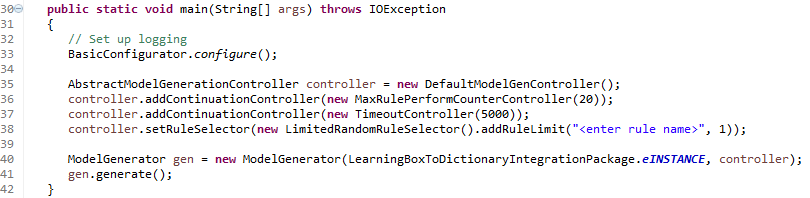
\includegraphics[width=1\textwidth]{eclipse_modelgen_stub.png}
\caption{Stub for the model generator}
\label{eclipse:modelgen}
\end{center}
\end{figure}

The \texttt{ModelGenerator} class uses an \texttt{AbstractModelGenerationController} to control the generation process (Line 35). 
In this default template the generation process will be terminated after 20 rules have been applied (\texttt{Max\-Rule\-Perform\-Counter\-Controller} (Line 36)). 
Additionally, the \texttt{Time\-out\-Con\-trol\-ler} will terminate the process after 5000ms (Line 37). 
You can use the \texttt{Max\-Model\-Size\-Controller} class to terminate the generation process if a specific model size has been reached. 
The \texttt{RuleSelector} controls which rules are selected as the next to be executed. 
The built-in \texttt{LimitedRandomRuleSelector} always selects a random rule and has the additional feature to limit the number of performs for specific rules (Line 38).
As with everything we generate, this is standard Java code, doesn't bite, and can be extended as you wish with your own controller classes and generation strategies.

\begin{itemize}

\item[$\blacktriangleright$]  To ensure that we only get a model with a single root, change \texttt{$<$enter rule name$>$} to \texttt{BoxToDictionaryRule} so that this island rule (which is always applicable) will only be applied once.

\item[$\blacktriangleright$] Save the file and hit \texttt{Run}!

You'll probably get some logging information in the console (\Cref{eclipse:modelgen_log}) containing information gathered during the generation process such as model size for each domain, number of performs for each rule, duration of generation process for each rule etc.

\end{itemize}


\begin{figure}[htbp]
\renewcommand\figurename{Figure} 
\begin{center}
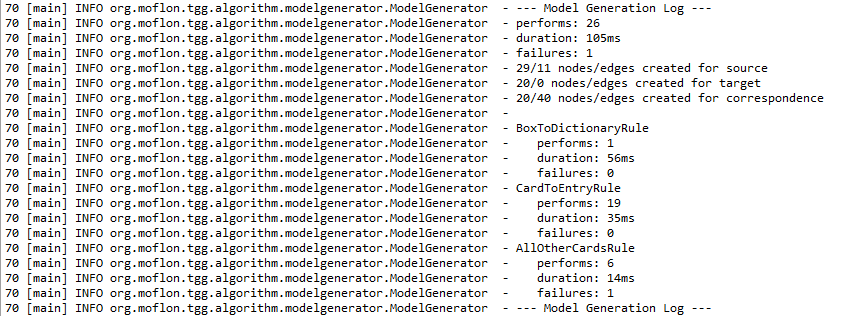
\includegraphics[width=1\textwidth]{eclipse_example_logging.png}
\caption{Logging output after model generation}
\label{eclipse:modelgen_log}
\end{center}
\end{figure}

In your \texttt{instances} folder there should now be a new folder named \texttt{generated\-Models} with a timestamp suffix. 
It contains your newly generated source and target models.
Have fun viewing.
Why not try creating like seriously gigantic models?

Note that to support model generation for custom attribute condition in general, you might have to specify additional \texttt{\#gen} adornments. 
No additional adornments were required for our new attribute condition, and all library conditions suppo

%%% Local Variables: 
%%% mode: latex
%%% TeX-master: "../src/TGG_mainFile"
%%% End: 
